\documentclass[../main.tex]{subfiles}
\graphicspath{{\subfix{../images/}}, {\subfix{../}}}

\begin{document}
\chapter{Coherence length and penetration depth in strongly correlated superconductors}\label{ch:coherence-length-and-penetration-depth-in-strongly-correlated-superconductors}

\todo{Put in source}

Order parameter (OP) of a superconducting condensate with FMP has the form
\begin{equation}
    \Psi_{\vb{q}} (\vb{r}) = \vert \Psi_{\vb{q}} \vert e^{i \vb{q} \vb{r}}
\end{equation}
where \(\vb{q}\) is the center-of-mass momentum of Cooper pairs.

FMP is well known from Fulde-Ferrel-Larkin-Ovchinnikov (FFLO) theory, where the single-momentum phase used here corresponds to FF-type pairing. \todo{What does that mean? More details on FFLO theory}

\section{Ginzburg-Landau description}

First: Motivate how the FMP constraint relates to \(\lambda_L\) and \(\xi_0\).

GL low-order expansion of the free energy density \(f_{\mathrm{GL}}\) in terms of the FMP-constrained OP reads
\begin{equation}
    1
\end{equation}
\todo{Fill in equation}
\todo{More details on GL theory in general}


The temperature dependent correlation length \(\xi\) appears as the natural length scale of the amplitude mode (\(\propto \alpha\)) and kinetic energy term
\begin{equation}
    \xi (T) =
\end{equation}
\todo{Fill in equation}
with the zero temperature value \(\xi_0\) being the coherence length.

%“length scale associated with this breakdown is ξ and can, therefore, be inferred from the q-dependent OP suppression √”

%“he q-dependent OP suppression. We employ, here, the criterion ξ = 1/(√2|Q|) with Q such that |ΨQ/Ψ0| = 1/√2 The finite cen”

%“| = finite center-of-mass momentum of the Cooper pairs is concomitant with the flow of a charge supercurrent jq ∝ ∂fGL/∂q ∝ |Ψq|2q This current density is a non”

%j“∝ ∝ || current density is a non-monotonous function of q with a maximum called depairing current density jdp”

%“jdp is related to the London penetration depth via λL(T) = s Φ0 3√3πµ0ξjdp = λL,0 1 − T Tc 4!− 2”
%“microscopic description, we acquire the OP and supercurrent density from the components of the Nambu-Gor’kov Green function G with FMP constraint. Nambu spinors † †”

%“G Nambu spinors ψ† k,q = (c† k+ q 2 ↑, c−k+ q 2 ↓) duced which”

%“corresponding Green function is a 2 × 2 matrix Gq(τ, k) = −⟨Tτψk,q(τ )ψ† k,q⟩ = Gq(τ, k) Fq(τ, k) F∗ q (τ, k) −Gq(−τ, −k)”

%“normal (anomalous) Green function G (F) components on imaginary time τ take over the q-dependence.”

%“local anomalous Green function |Ψq| ≡ [Floc q (τ = 0−)]αα = X k ⟨cαk+ q 2 ↑cα−k+ q 2 ↓⟩” From microscopic treatment we get order parameter, the from that we get penetration depth and coherence length in GL theory?

\section{Phase transitions and broken symmetry}

Following~\cite[ch. 11]{colemanIntroductionManyBodyPhysics2015}.

\subsection{Order parameter concept}

Landau theory: phase transitions (e.g.\ iron becomes magnetic, water freezes, superfluidity/superconductivity) are associated with the development of an order parameter when the temperature drops below the transition temperature \(T_C\) \todo{This works also for phase transitions not dependent of temperatures, so e.g.\ in pressures?}
\begin{equation}
    \vert \psi \vert =
    \begin{cases}
        0\;,\; T > T_C \\
        \vert \psi_0 \vert > 0 \;,\; T < T_C
    \end{cases}
\end{equation}
Landau theory does not need microscopic expression for order parameter, it provides corse-grained description of the properties of matter.
The order parameter description is good at length scales above \(\xi_0\), the coherence length (e.g.\ size of Cooper pairs for SC).

\subsection{Landau theory}

Landau theory

Going from a one to a \(n\)-component order parameters, we can actually

Particularly important example: complex or two component order parameter in superfluids and superconductors:
\begin{equation}
    \psi = \psi_1 + \iu \psi_2 = \vert \psi \vert e^{\iu \phi}
\end{equation}
The Landau free energy takes the form:
\begin{equation}
    f[\psi] = r(\psi^* \psi) + \frac{u}{2} (\psi^* \psi)^2
\end{equation}
Figure~\ref{fig:Landau free energy mexican hat potential} shows the Landau free energy as function of \(\psi\).

\begin{figure}[t]
    \centering
    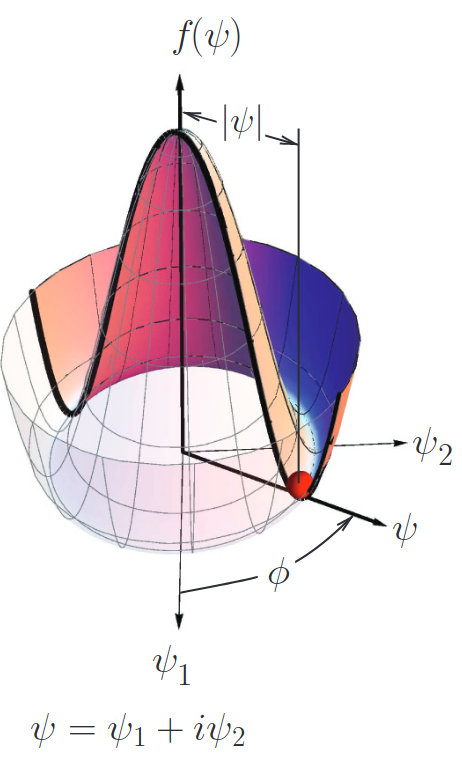
\includegraphics[width=0.3\textwidth]{images/landau free energy mexican hat}
    \caption{Mexican hat potential}
    \label{fig:Landau free energy mexican hat potential}
\end{figure}

In this `Mexican hat' potential: order parameter can be rotated continuously from one broken-symmetry state to another.
If we want the phase to be rigid, we need to introduce an
There is a topological argument for the fact that the phase is rigid.
This leads to Ginzburg-Landau theory.
Will see later: well-defined phase is associated with persistent currents or superflow.

\subsection{Ginzburg-Landau theory I: Ising order}

\todo{Short introduction for one-component order parameter, so the connection to complex order parameters gets clear}

\subsection{Ginzburg-Landau theory II: complex order and superflow}

Now: G-L theory of complex or two-component order parameters, so superfluids and superconductors.
Heart of discussion: emergence of a `macroscopic wavefunction', where the microscopic field operators \(\hat{\psi(x)}\) acquire an expectation value:
\todo{What exactly are field operators again?}
\begin{equation}
    \braket{\psi (x)} = \psi (x) = \vert \psi (x) \vert e^{\iu \theta(x)}
\end{equation}
Magnitude determines density of particles in the superfluid:
\begin{equation}
    \vert \psi(x) \vert^2 = n_s (x)
\end{equation}
\todo{More info on that? Does that come later in chapter?}
Twist/gradient of phase determines superfluid velocity:
\begin{equation}
    \vb{v}_s (x) = \frac{\hbar}{m} \Delta \phi (x)
\end{equation}
We will derive this later in the chapter.
Counterintuitive from quantum mechanics: GL suggested that \(\Phi(x)\) is a macroscopic manifestation of a macroscopic number of particles condensed into precisely the same quantum state.
Emergent phenomenon, collective properties of mater not a-priori self-evident from microscopic physics.

\todo{Here: rest of notes from Goodnotes}

\todo{Coherent states/Interpretation of states/Off-diagonal long-range order}

Phase rigidity and superflow: in GL theory, energy is sensitive to a twist of the phase.
Substitute \(\psi = \vert \psi \vert e^{\iu \phi}\) into GL free energy, gradient term is:
\begin{equation}
    \Delta \psi = ()
\end{equation}

\todo{Here: particle-current operator, especially for coherent state, connection with phase twist}

\subsection{Ginzburg-Landau theory III: charged fields}

\todo{Here: Meissner effect, etc}

\end{document}